\documentclass[final,11pt,oneside,UTF8]{report}
\usepackage{ctex}
\usepackage{float}
\usepackage{geometry}
\usepackage{graphicx}
\usepackage{mhchem}
\usepackage{amsmath,amsfonts,amssymb}
\title{碱式碳酸铜制备实验报告}
\author{AndyShen2006}
\date{Apr.29th.2021}
\begin{document}
\maketitle
\section{第一次实验}
\subsection{实验方案}
\paragraph{
    考虑使用硫酸铜法制取碱式碳酸铜(药品只有硫酸铜和碳酸氢钠。。。)\\
    反应方程式:
    %    $$2CuSO_4 \cdot 5H_2 O + 4NaHCO_3 = CuCO_3 \cdot Cu(OH)_2 \downarrow + 2Na_2 SO_4 + 3CO_2 \uparrow + 11H_2 O$$
    $$\ce{2CuSO4 * 5H2O + 4NaHCO3 -> CuCO3 * Cu(OH)2 v + 2Na2SO4 + 3CO2 ^ + 11H2O}$$
    这个反应在常温下就可以进行,但是产物不纯,如图所示
}
\begin{center}
    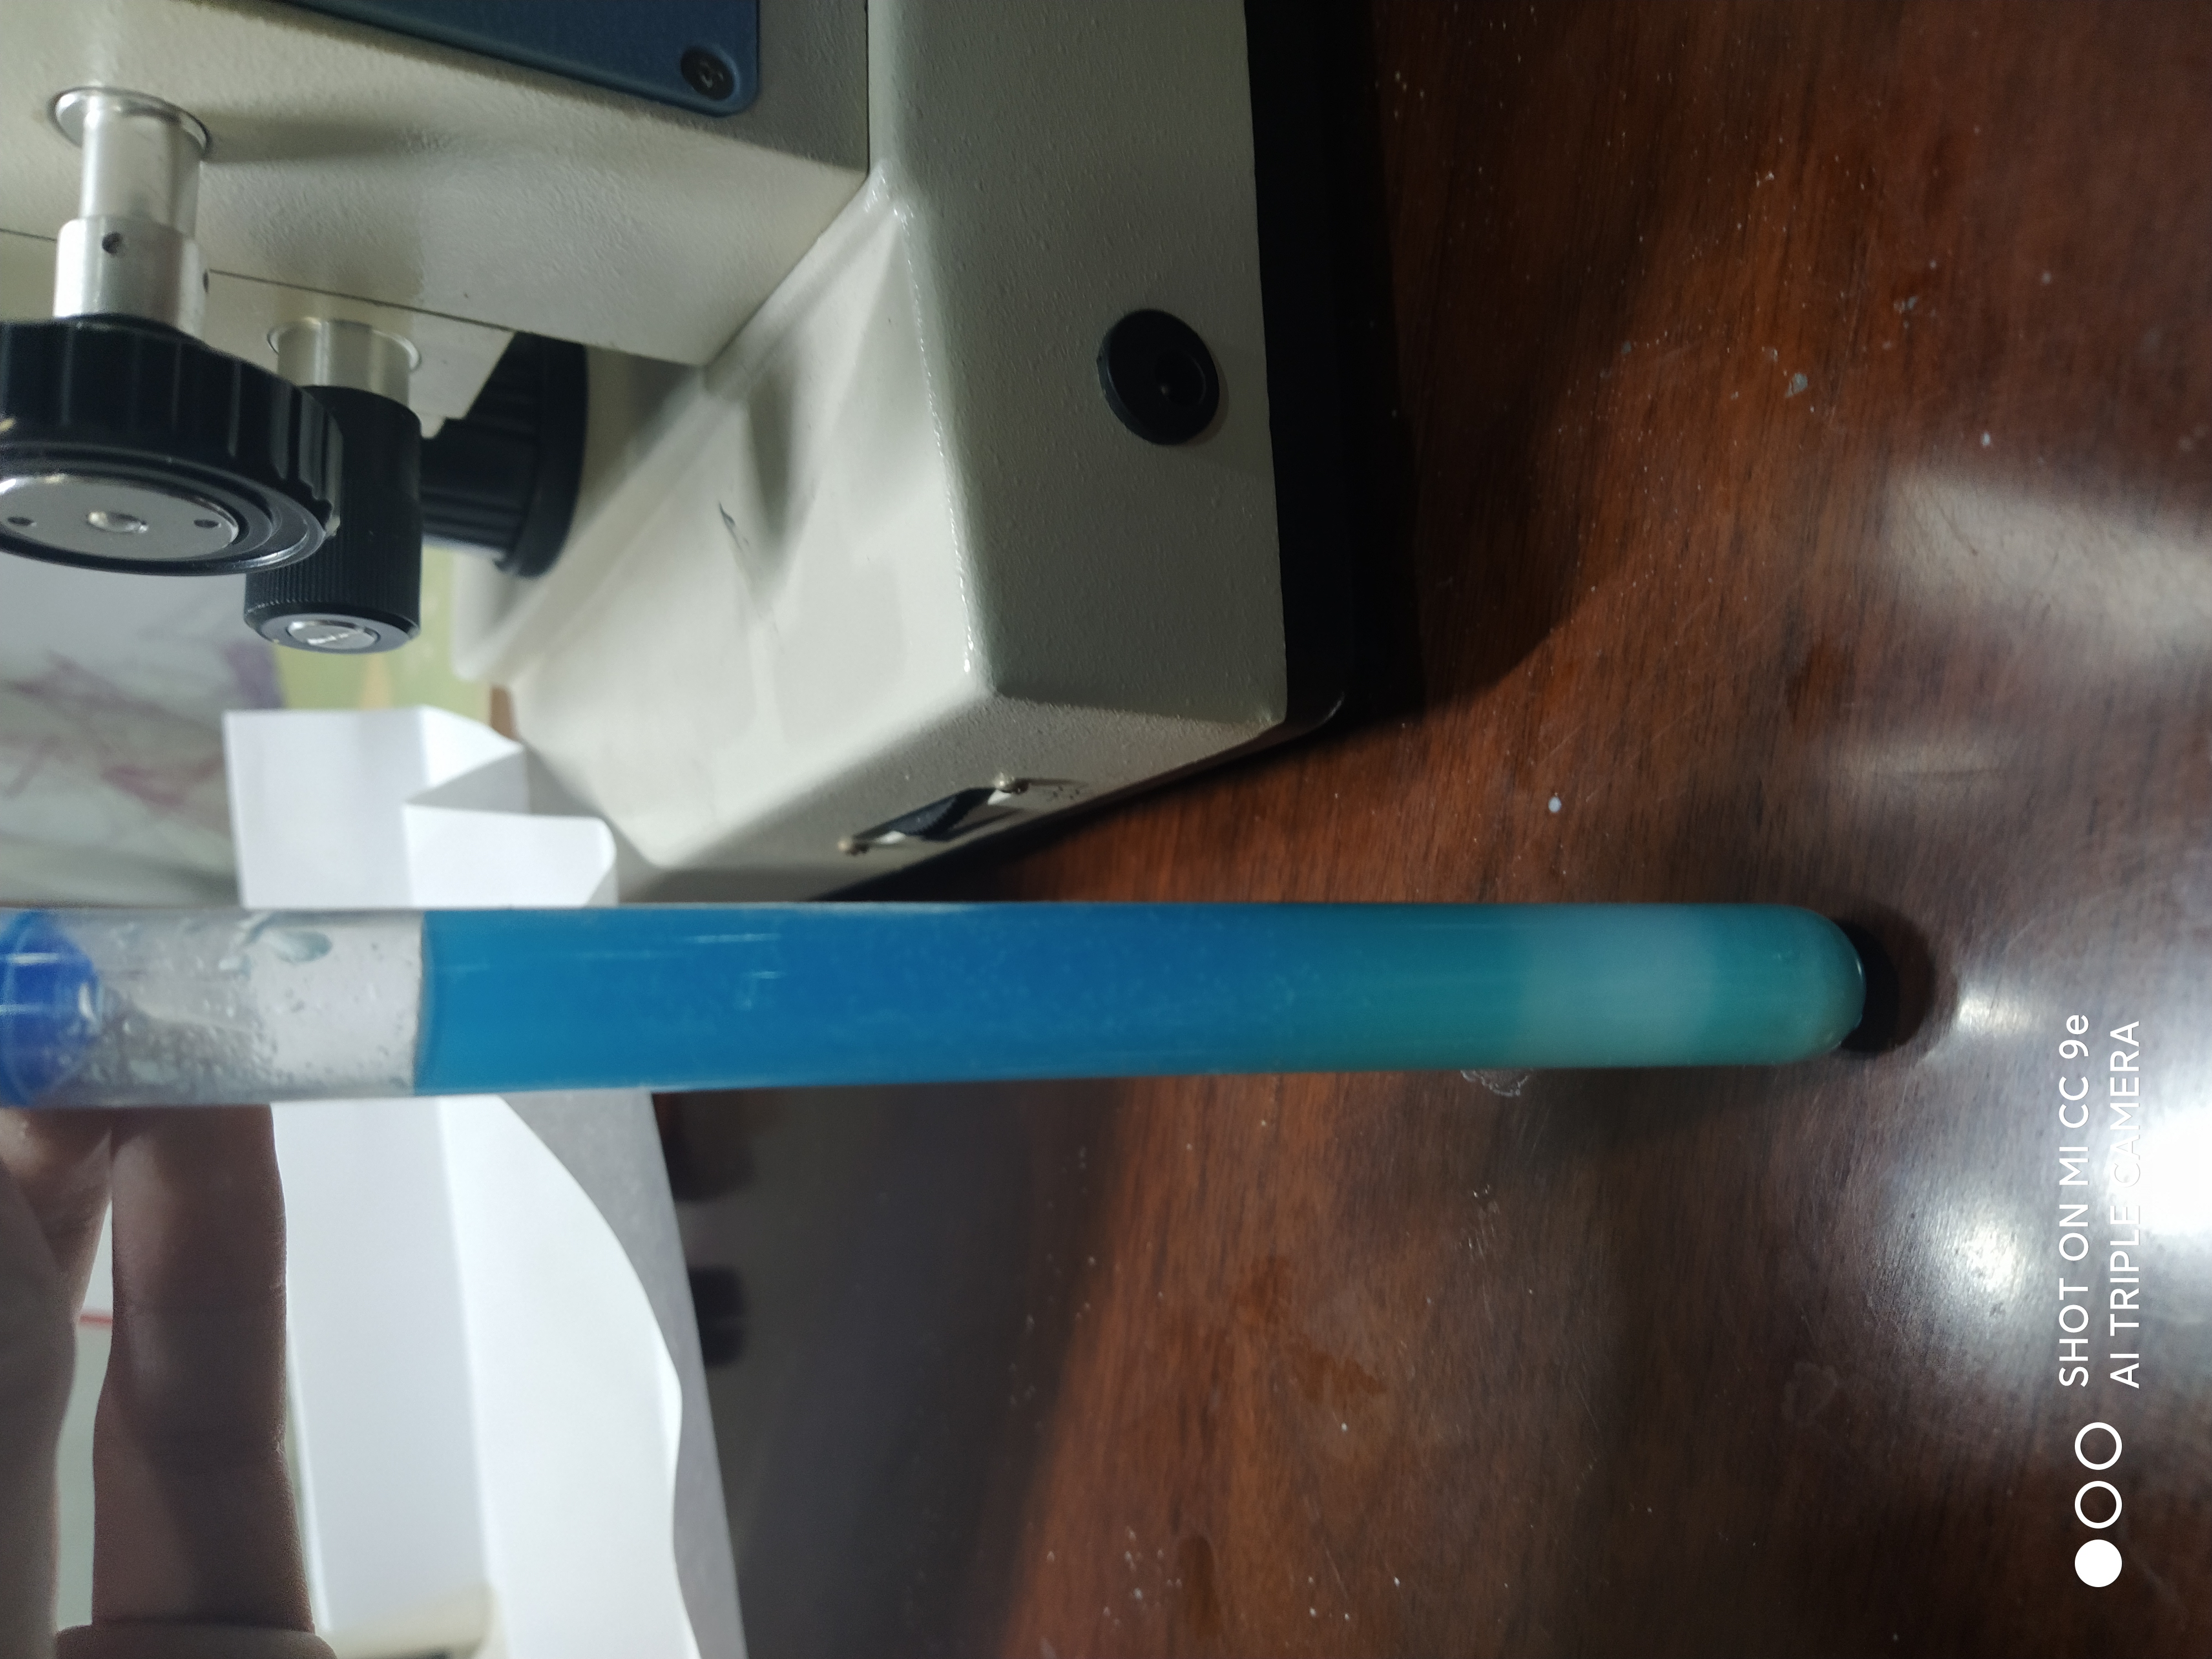
\includegraphics[scale=0.06,angle=-90]{photos/begin(lose).jpg}
\end{center}
\paragraph{
    因为产物不纯,颜色发蓝,故采取精确实验,并且在加热条件下充分进行。
    查表,计算质量,易知:\\
    1mol五水硫酸铜和2mol碳酸氢钠可以充分反应,五水硫酸铜相对分子质量为250,碳酸氢钠相对分子质量84
    故250g五水硫酸铜和168g碳酸氢钠可以充分反应,查表得知硫酸铜20摄氏度溶解度20.7g,碳酸氢钠溶解度
    9.6g,我调配了0.1mol/L的硫酸铜溶液和0.2mol/L的碳酸氢钠溶液。
}
\subsection{实验操作及现象}
\paragraph{
    将1g五水硫酸铜溶解至40mL水中\\
    将2g碳酸氢钠溶解至125mL水中,先倒入反应容器10mL。\\
}
\begin{center}
    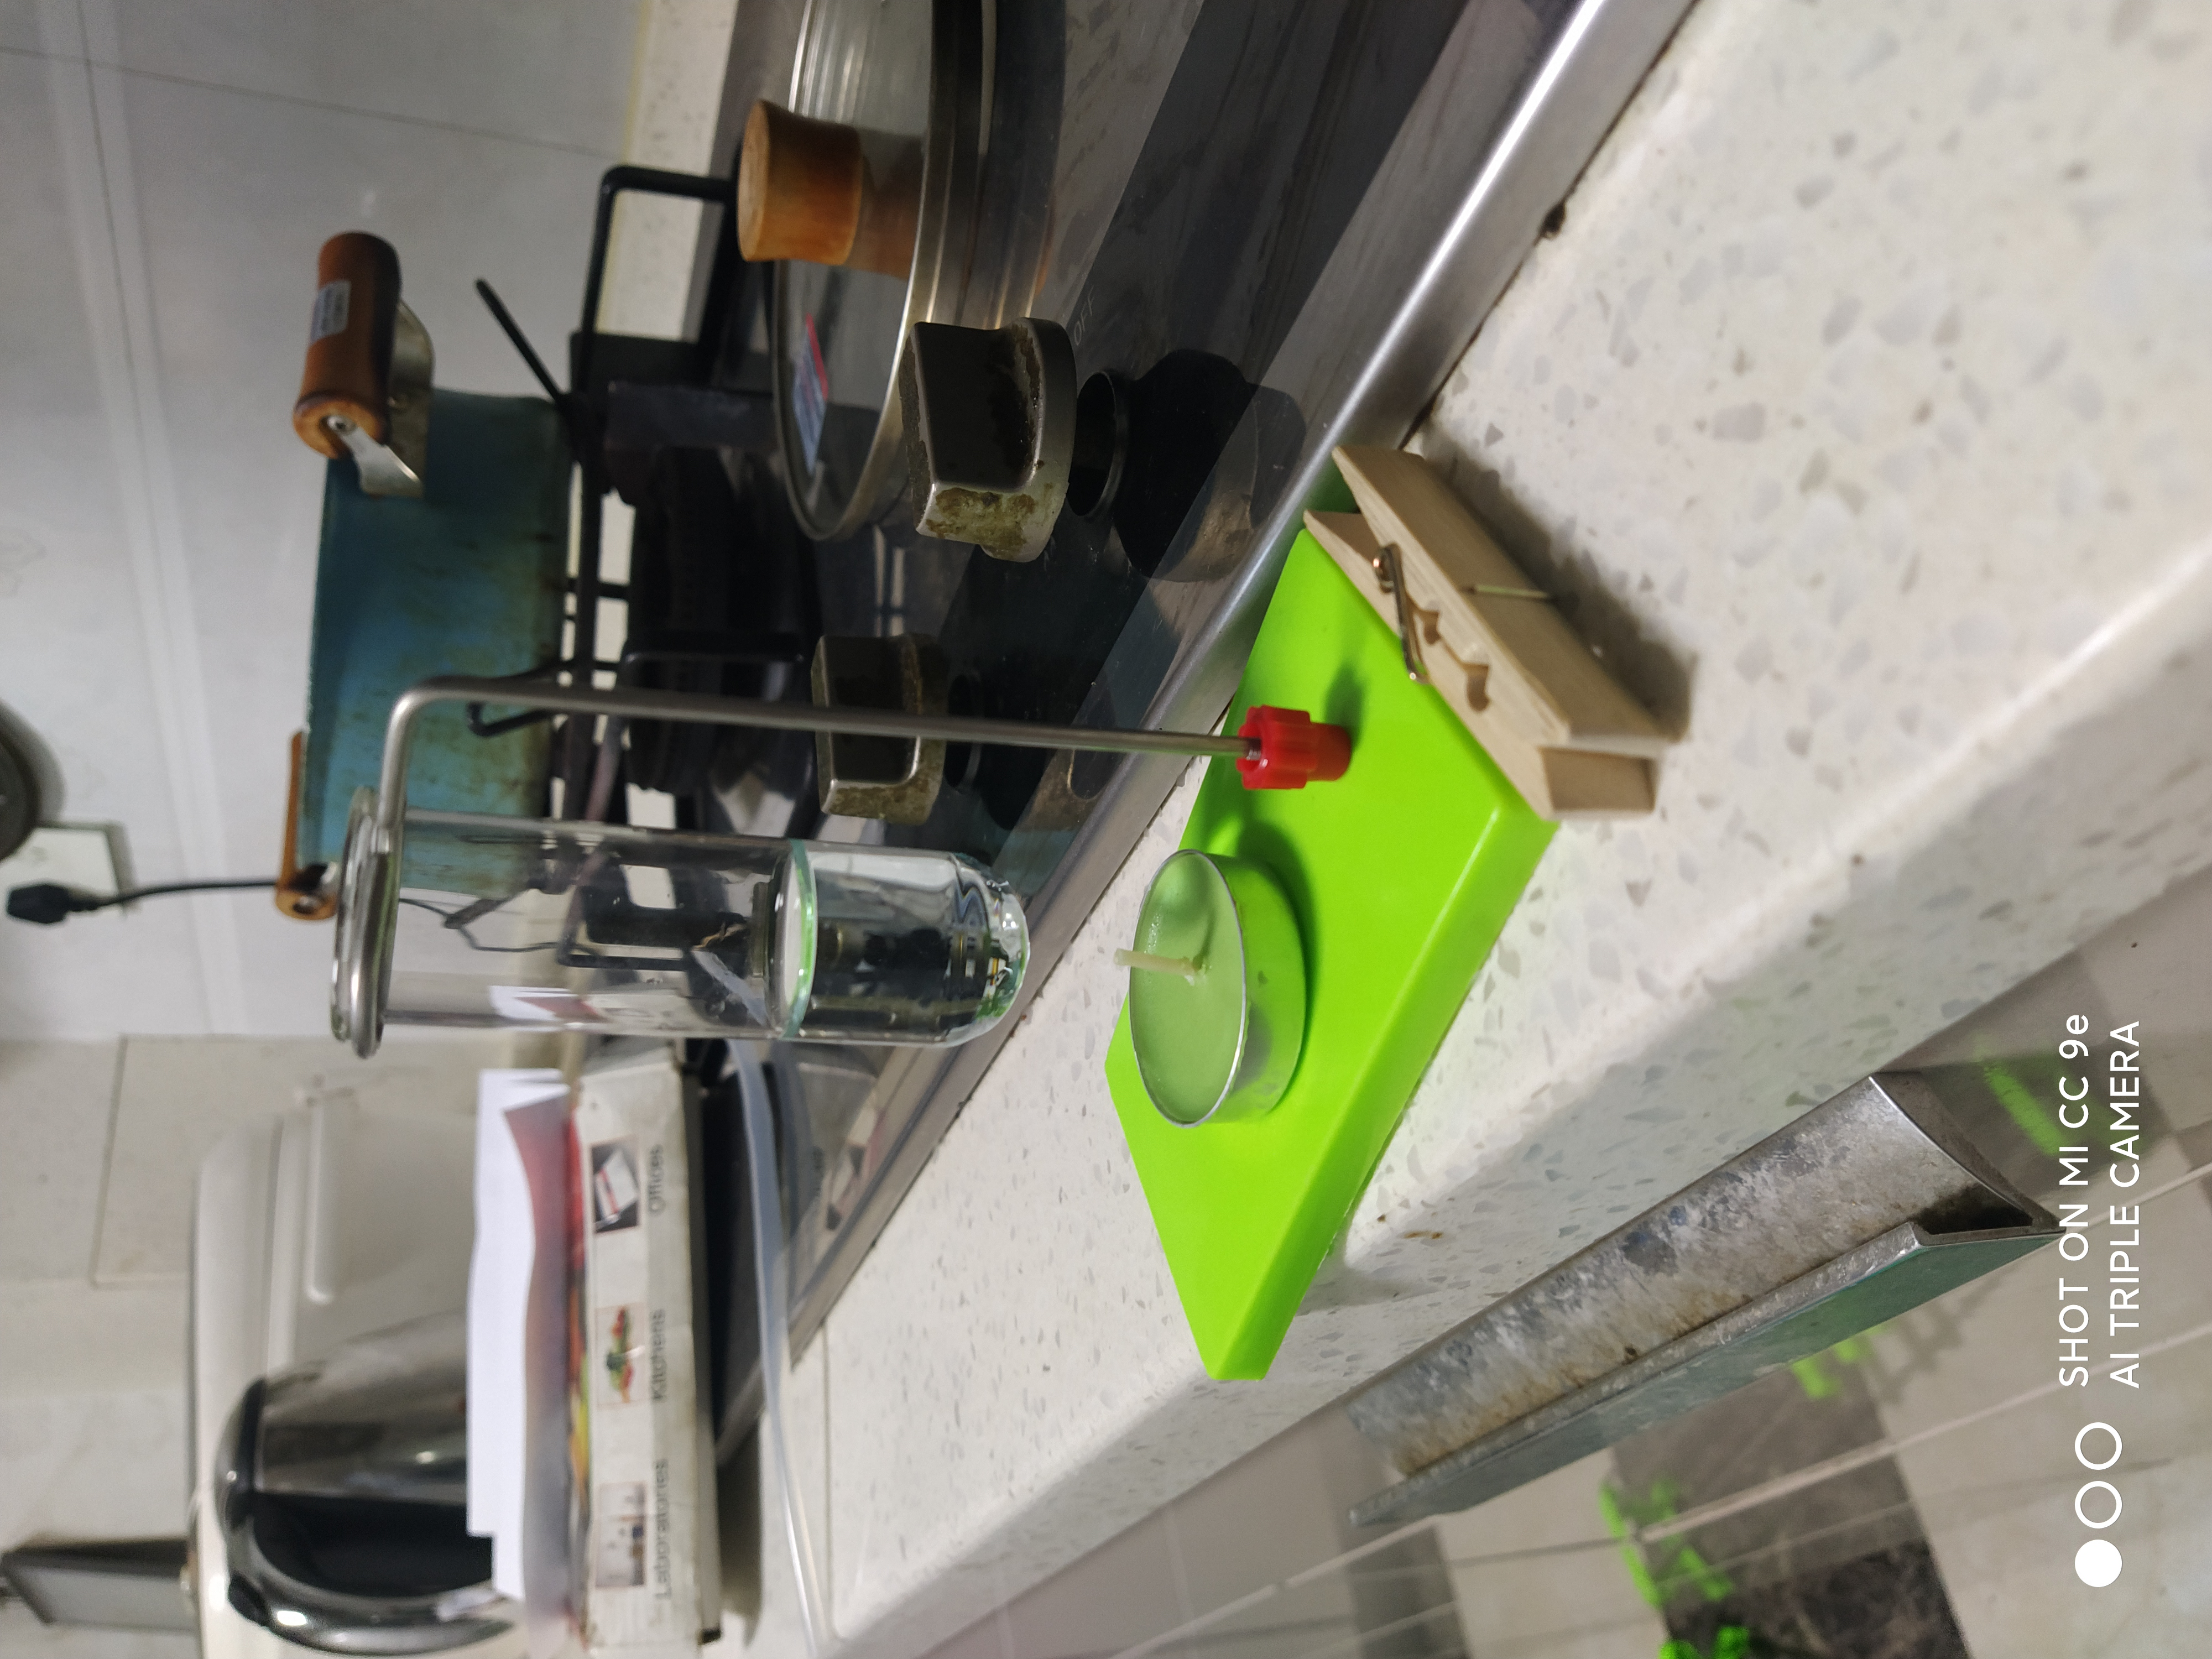
\includegraphics[scale=0.06,angle=-90]{photos/1Begin.jpg}
\end{center}
\paragraph{
    加热反应容器,同时在搅拌下将硫酸铜倒入反应容器10mL。\\
    用蜡烛一直加热,如果水少了就补一些,直至碱式碳酸铜沉淀不再被反应生成的二氧化碳托起,反应结束。\\
    反应过程中,试管一直发出爆裂声,应当是反应产生的二氧化碳所致。反应生成溶液,
    从开始的淡蓝色,慢慢的变成淡青色,最后变成黑色浑浊液体\\
}
\begin{center}
    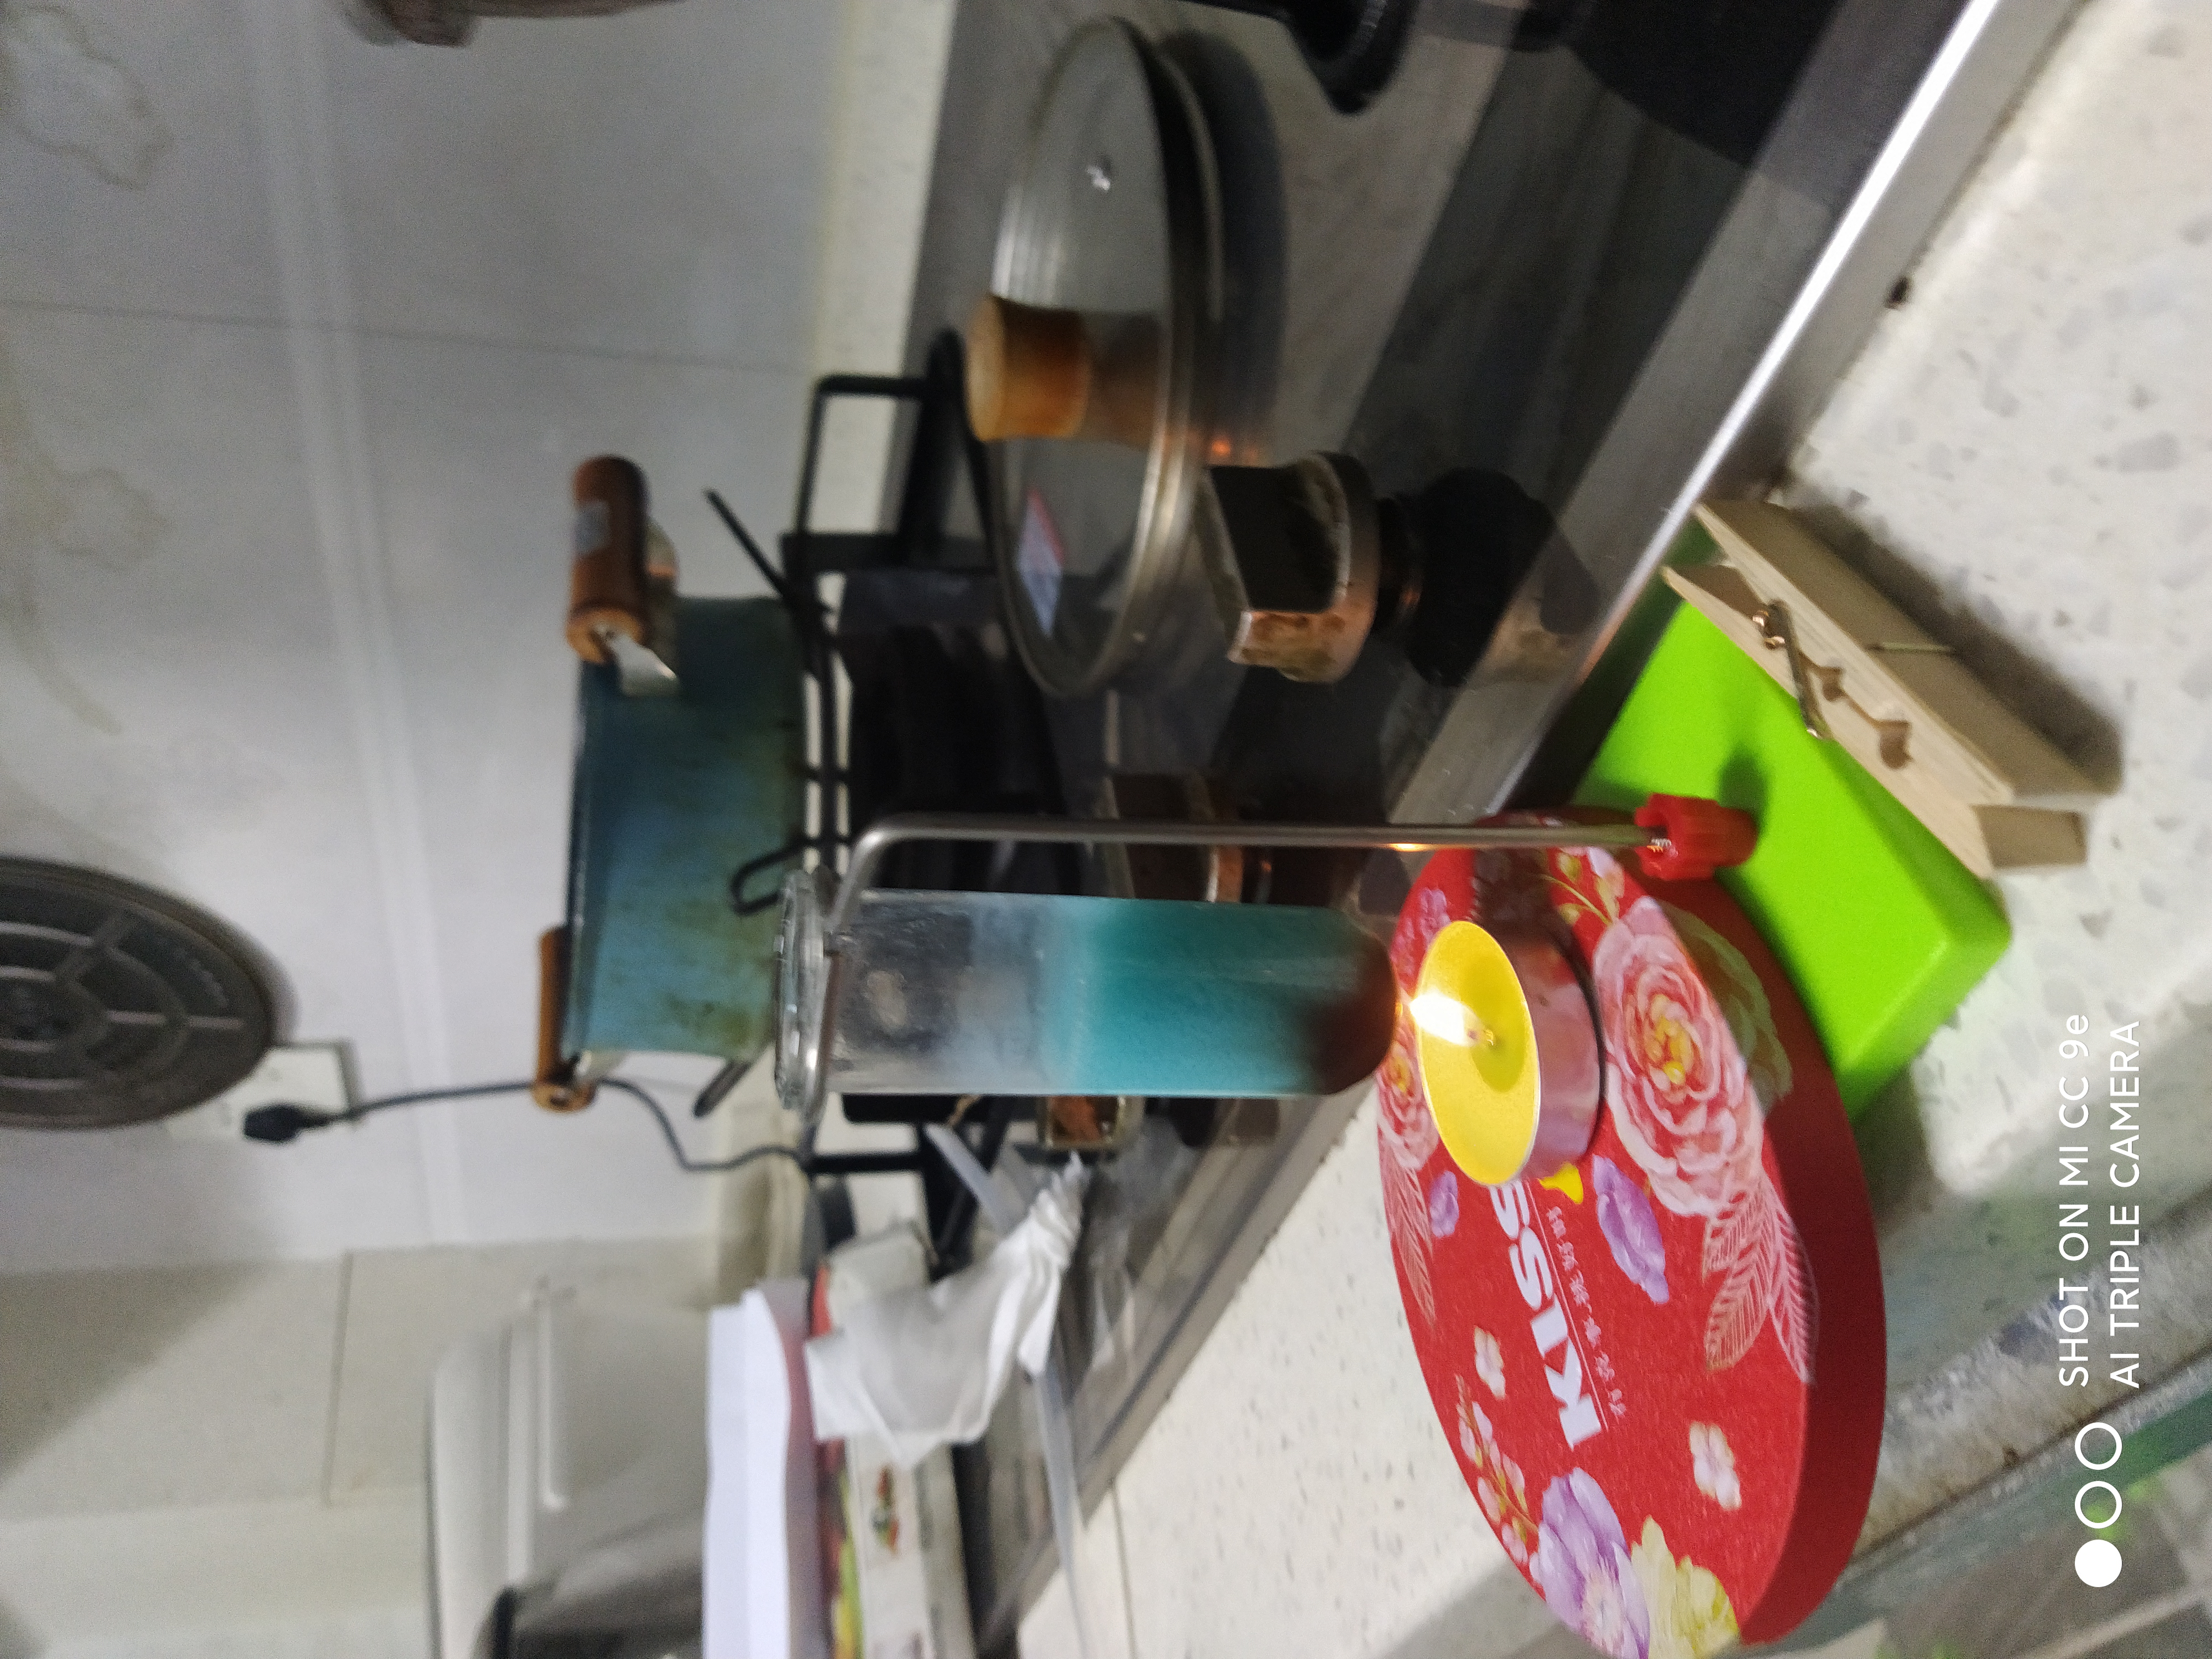
\includegraphics[scale=0.06,angle=-90]{photos/1During.jpg}
\end{center}
\paragraph{
    反应约进行了60分钟。\\
    反应结束时,上部黑色可能是受热不均的反应物分解所致。\\
}
\begin{center}
    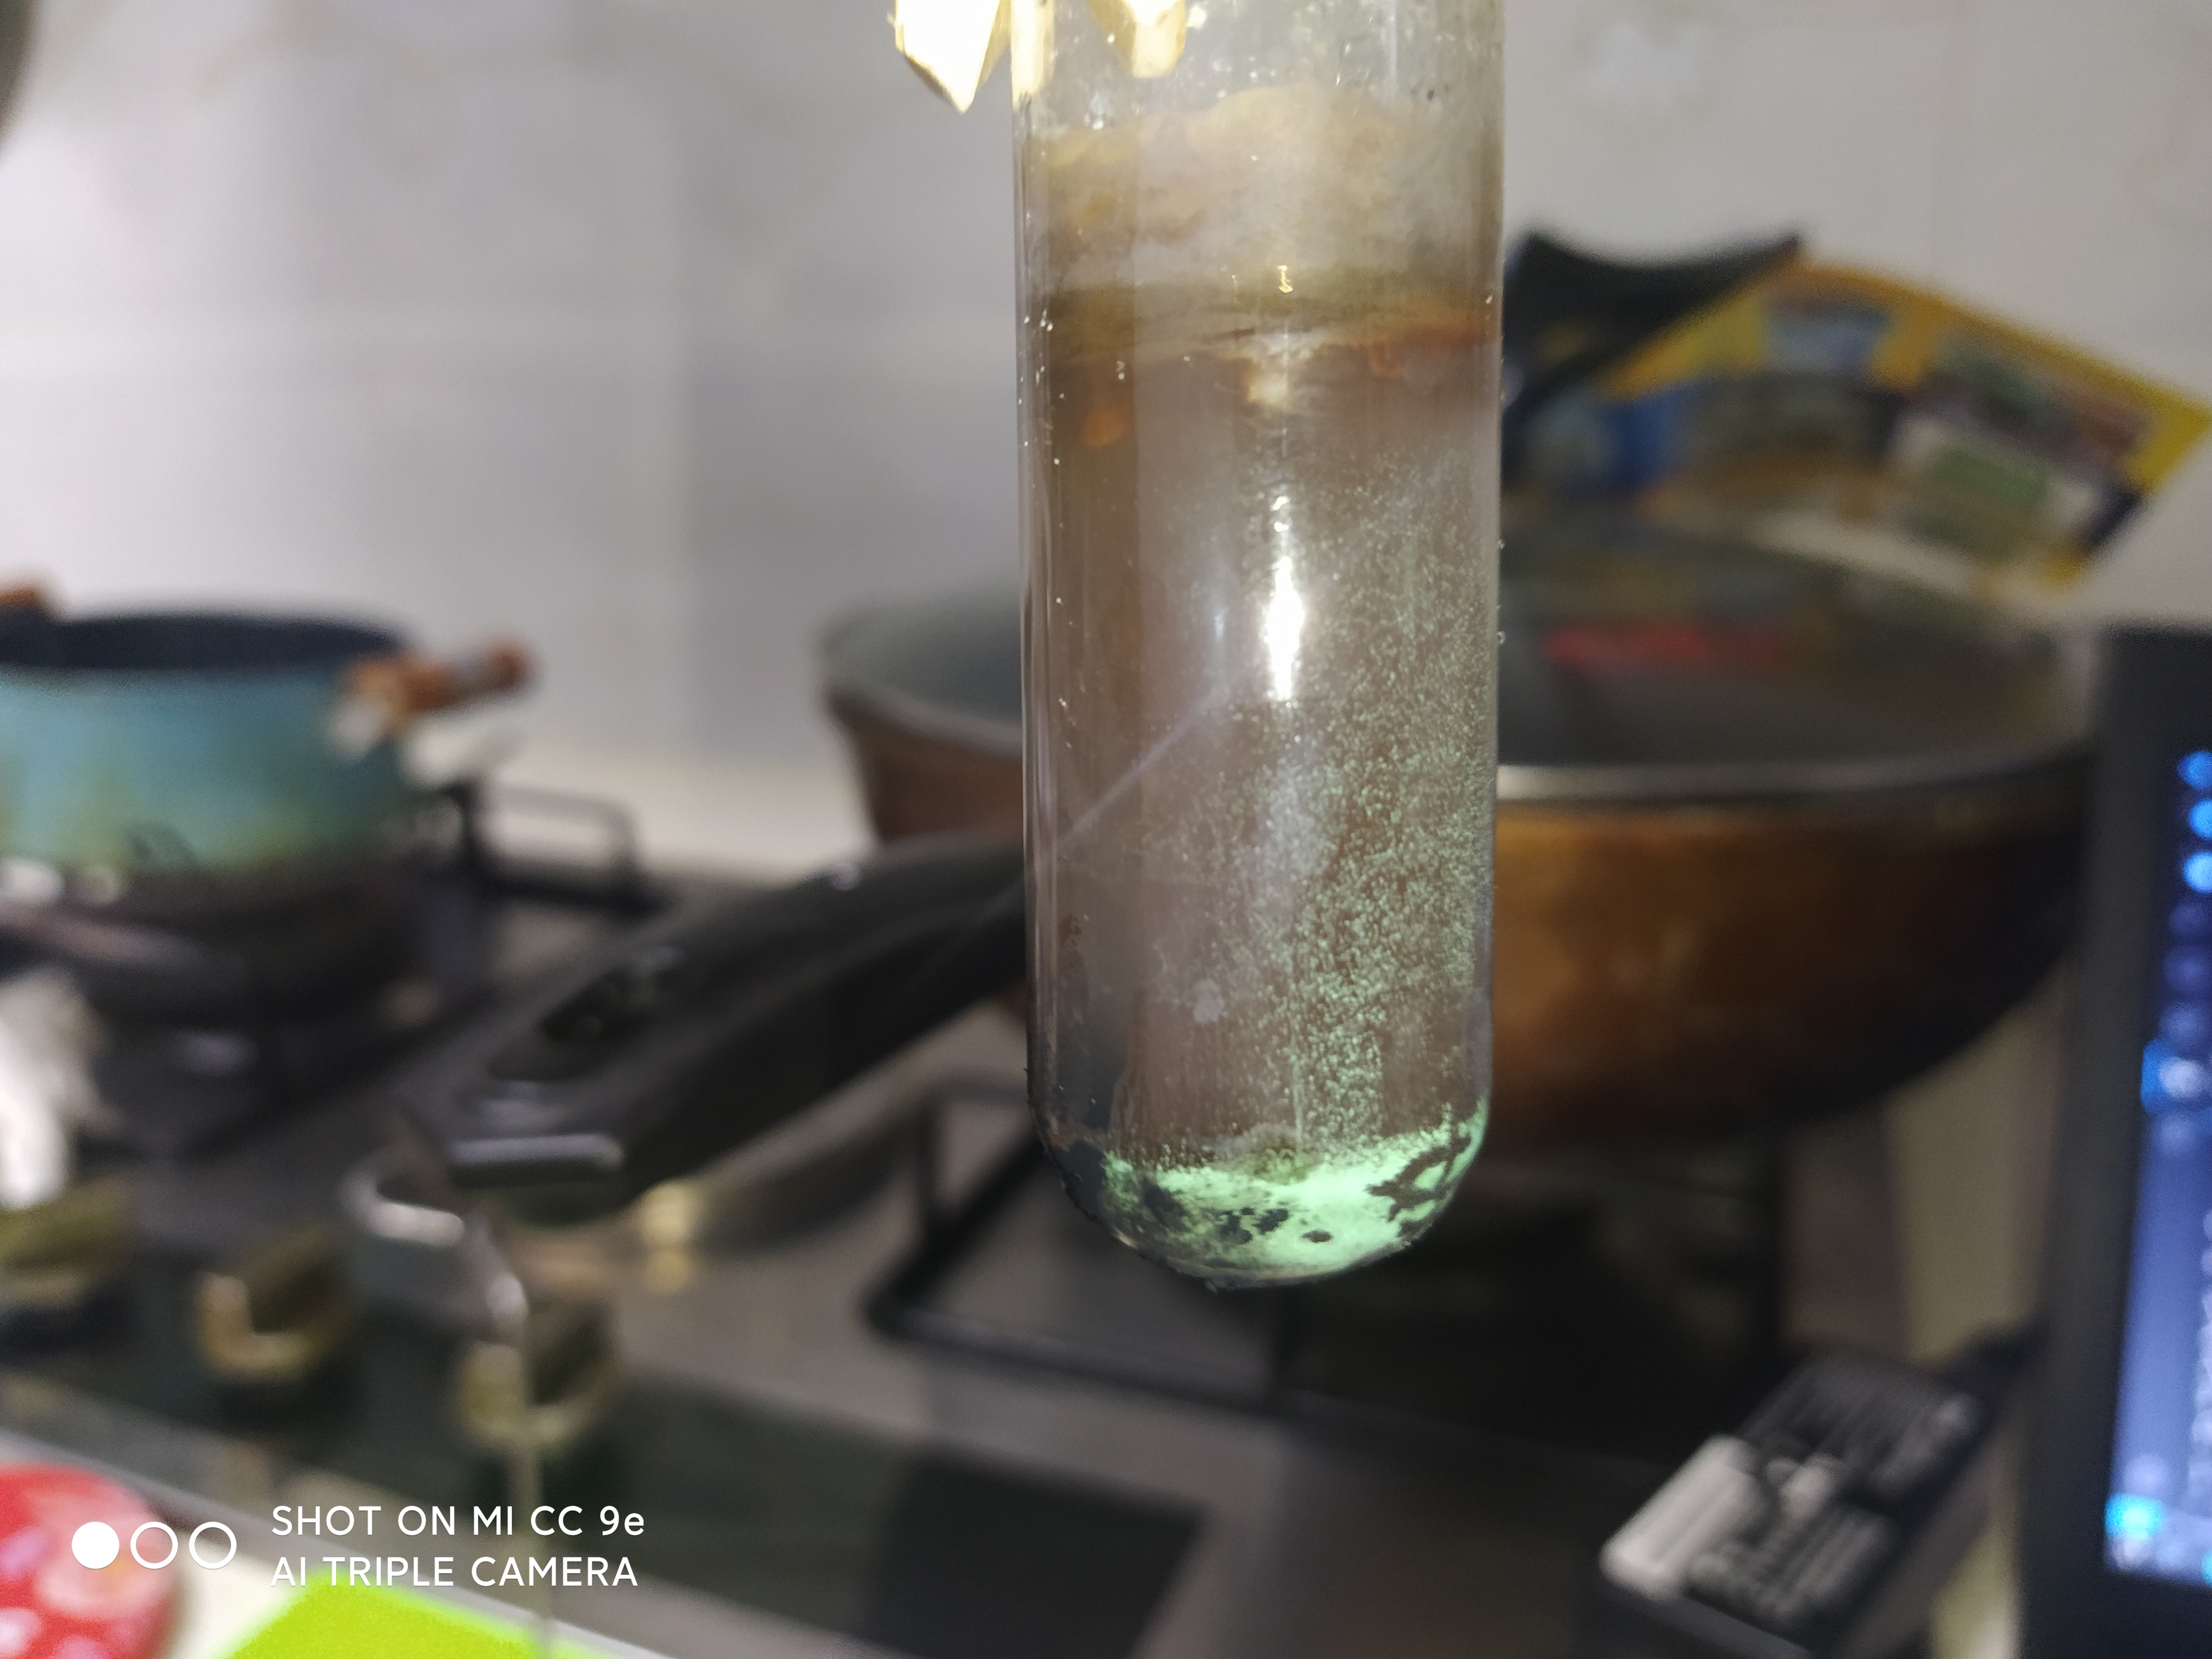
\includegraphics[scale=0.03]{photos/1End.jpg}
\end{center}
\subsection{实验总结}
\paragraph{
    因反应物过少,故生成物过少,无法定量检验产率,且不明黑色产物是否为反应物分解所致。
    故第二次实验,将增加反应物,且使用水浴加热。
}
\section{第二次实验}
\subsection{实验方案}
\paragraph{
    由于第一次量太少,无法检验产率,且未用水浴导致有杂质产生,故进行第二次实验\\
    本次增大溶液浓度,变为0.5mol/L硫酸铜溶液和1mol/L碳酸氢钠溶液反应,并且在水浴条件
    下进行\\
}
\subsection{实验操作及现象}
\paragraph{
    将12.5g五水硫酸铜溶解至100mL水中,将溶液放置备用。\\
    将10g碳酸氢钠溶解至100mL水中,并加入反应容器\\
}
\begin{center}
    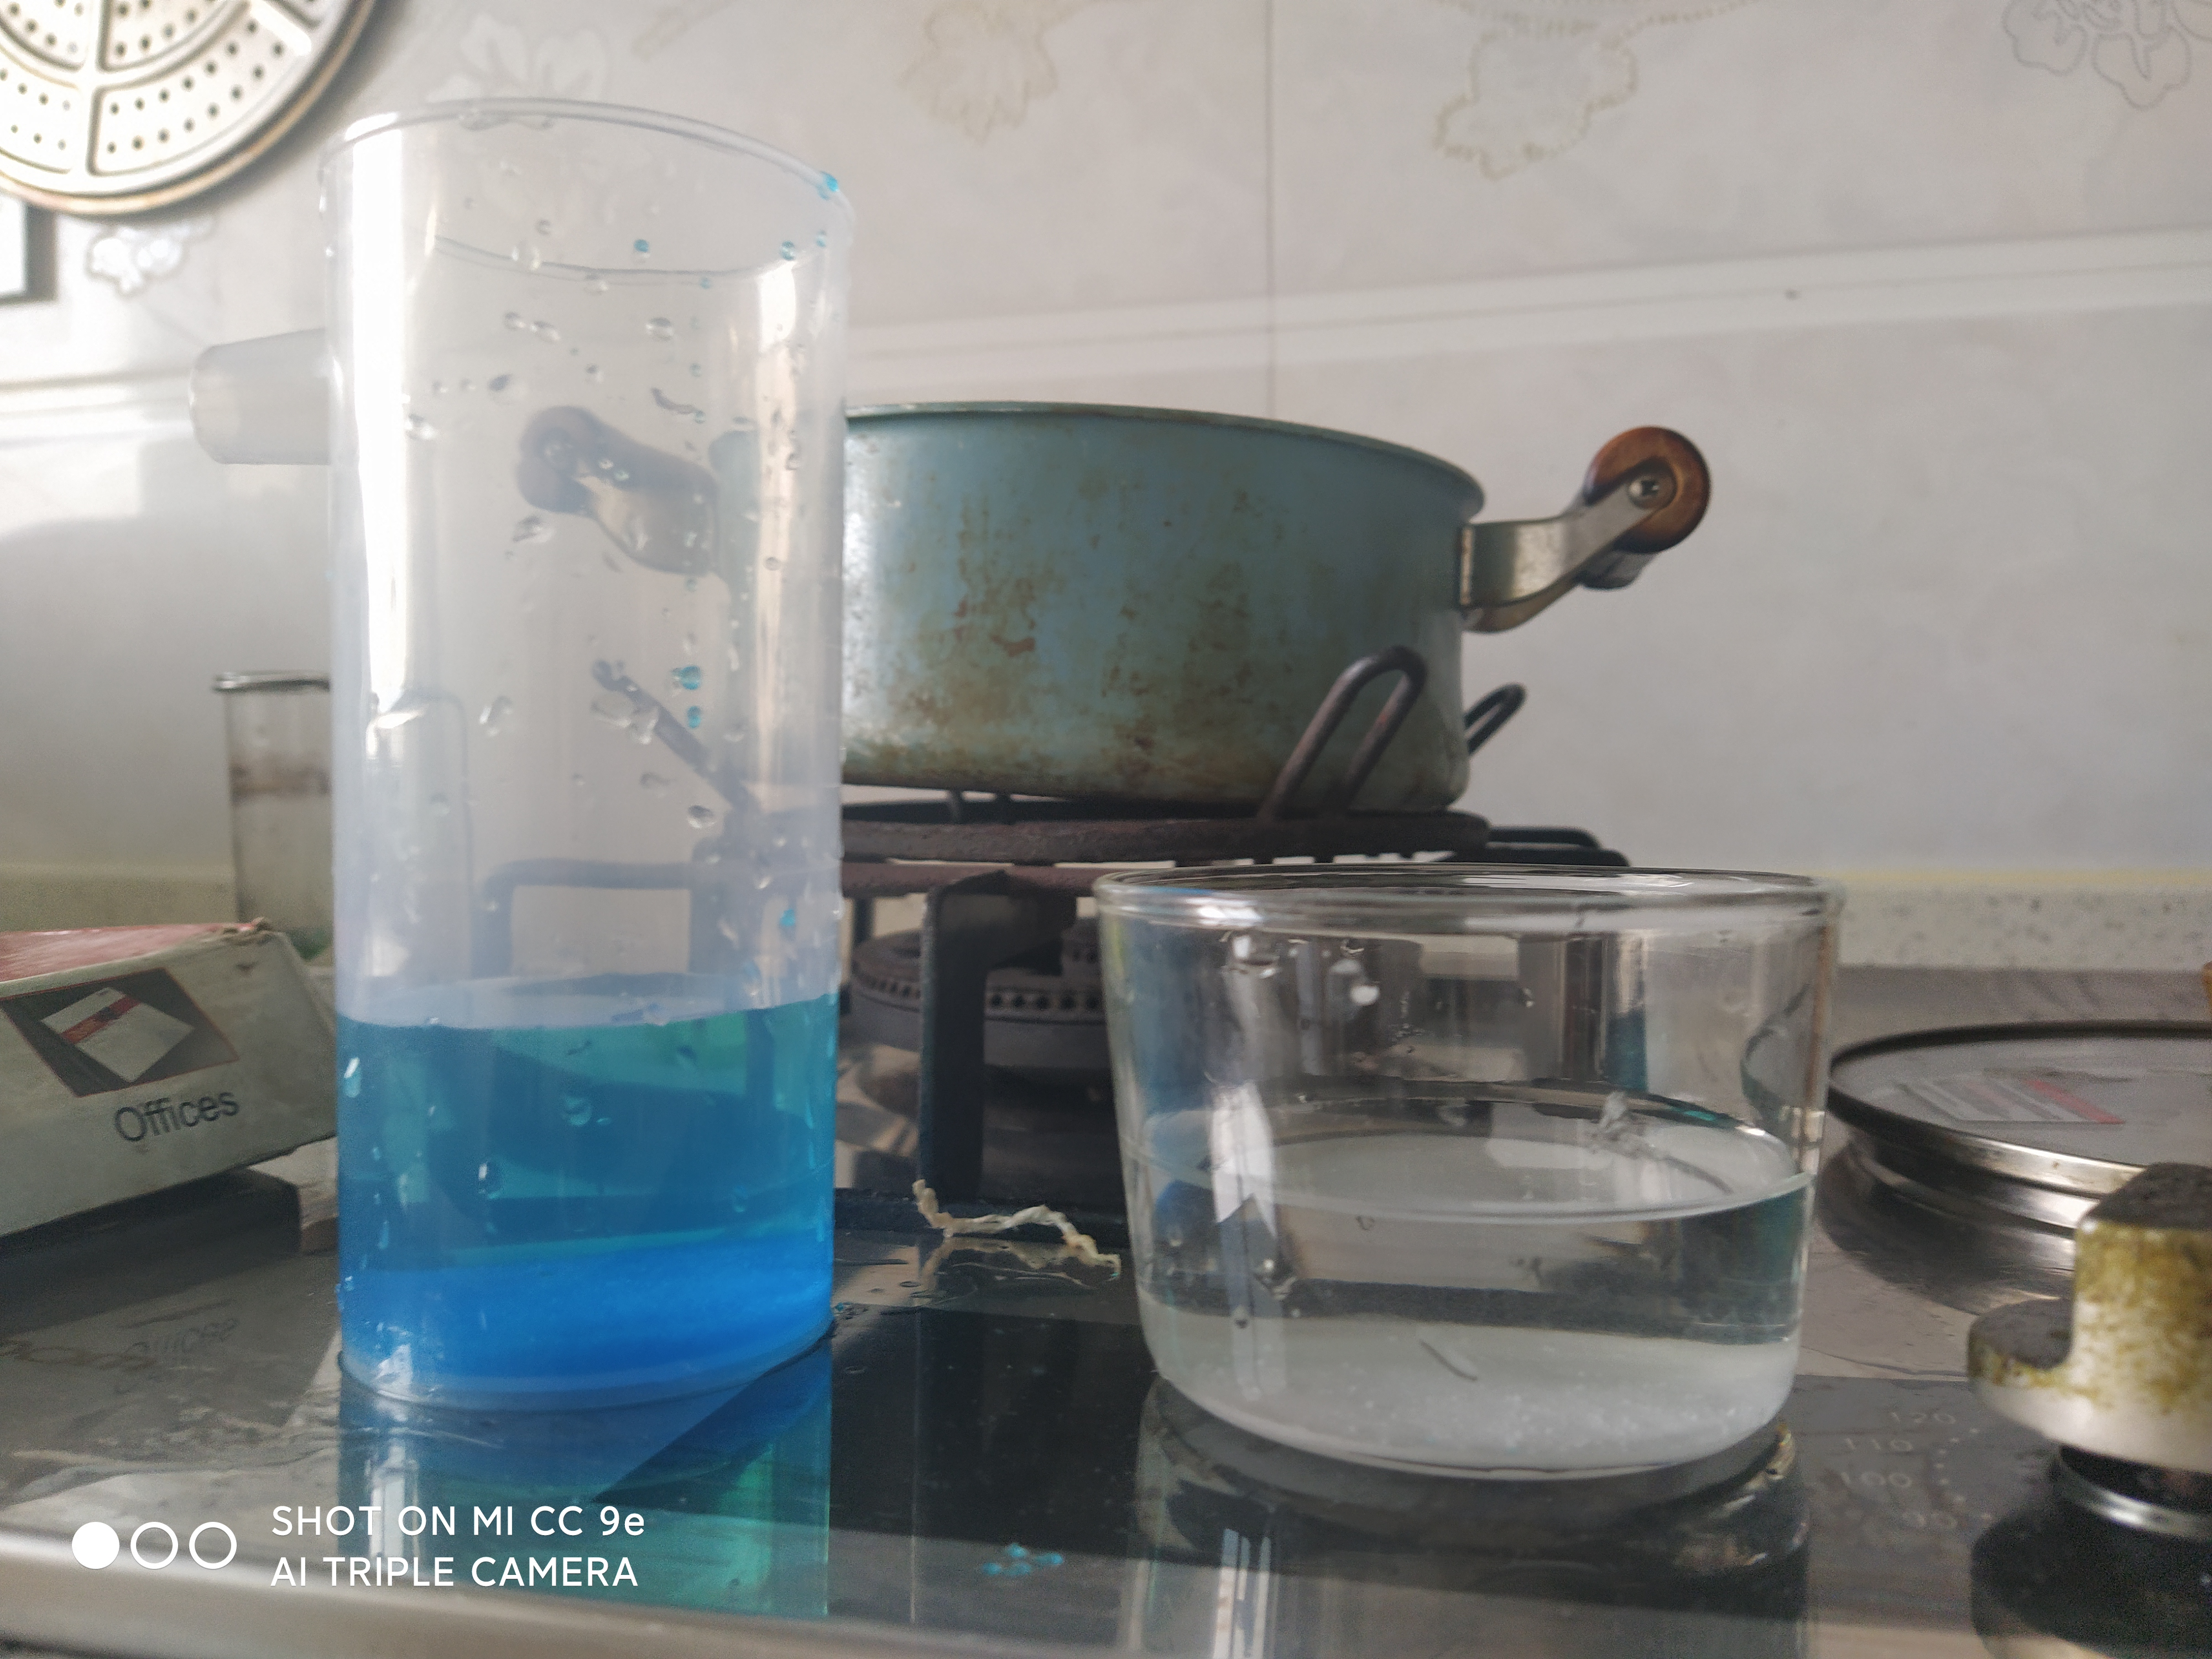
\includegraphics[scale=0.06]{photos/2Begin1.jpg}
\end{center}
\paragraph{
    水浴加热反应容器,至底部碳酸氢钠基本溶解为止,开始加入硫酸铜溶液反应。\\
    反应过程中有溶液扑出,故反应产率会略低\\
}
\begin{center}
    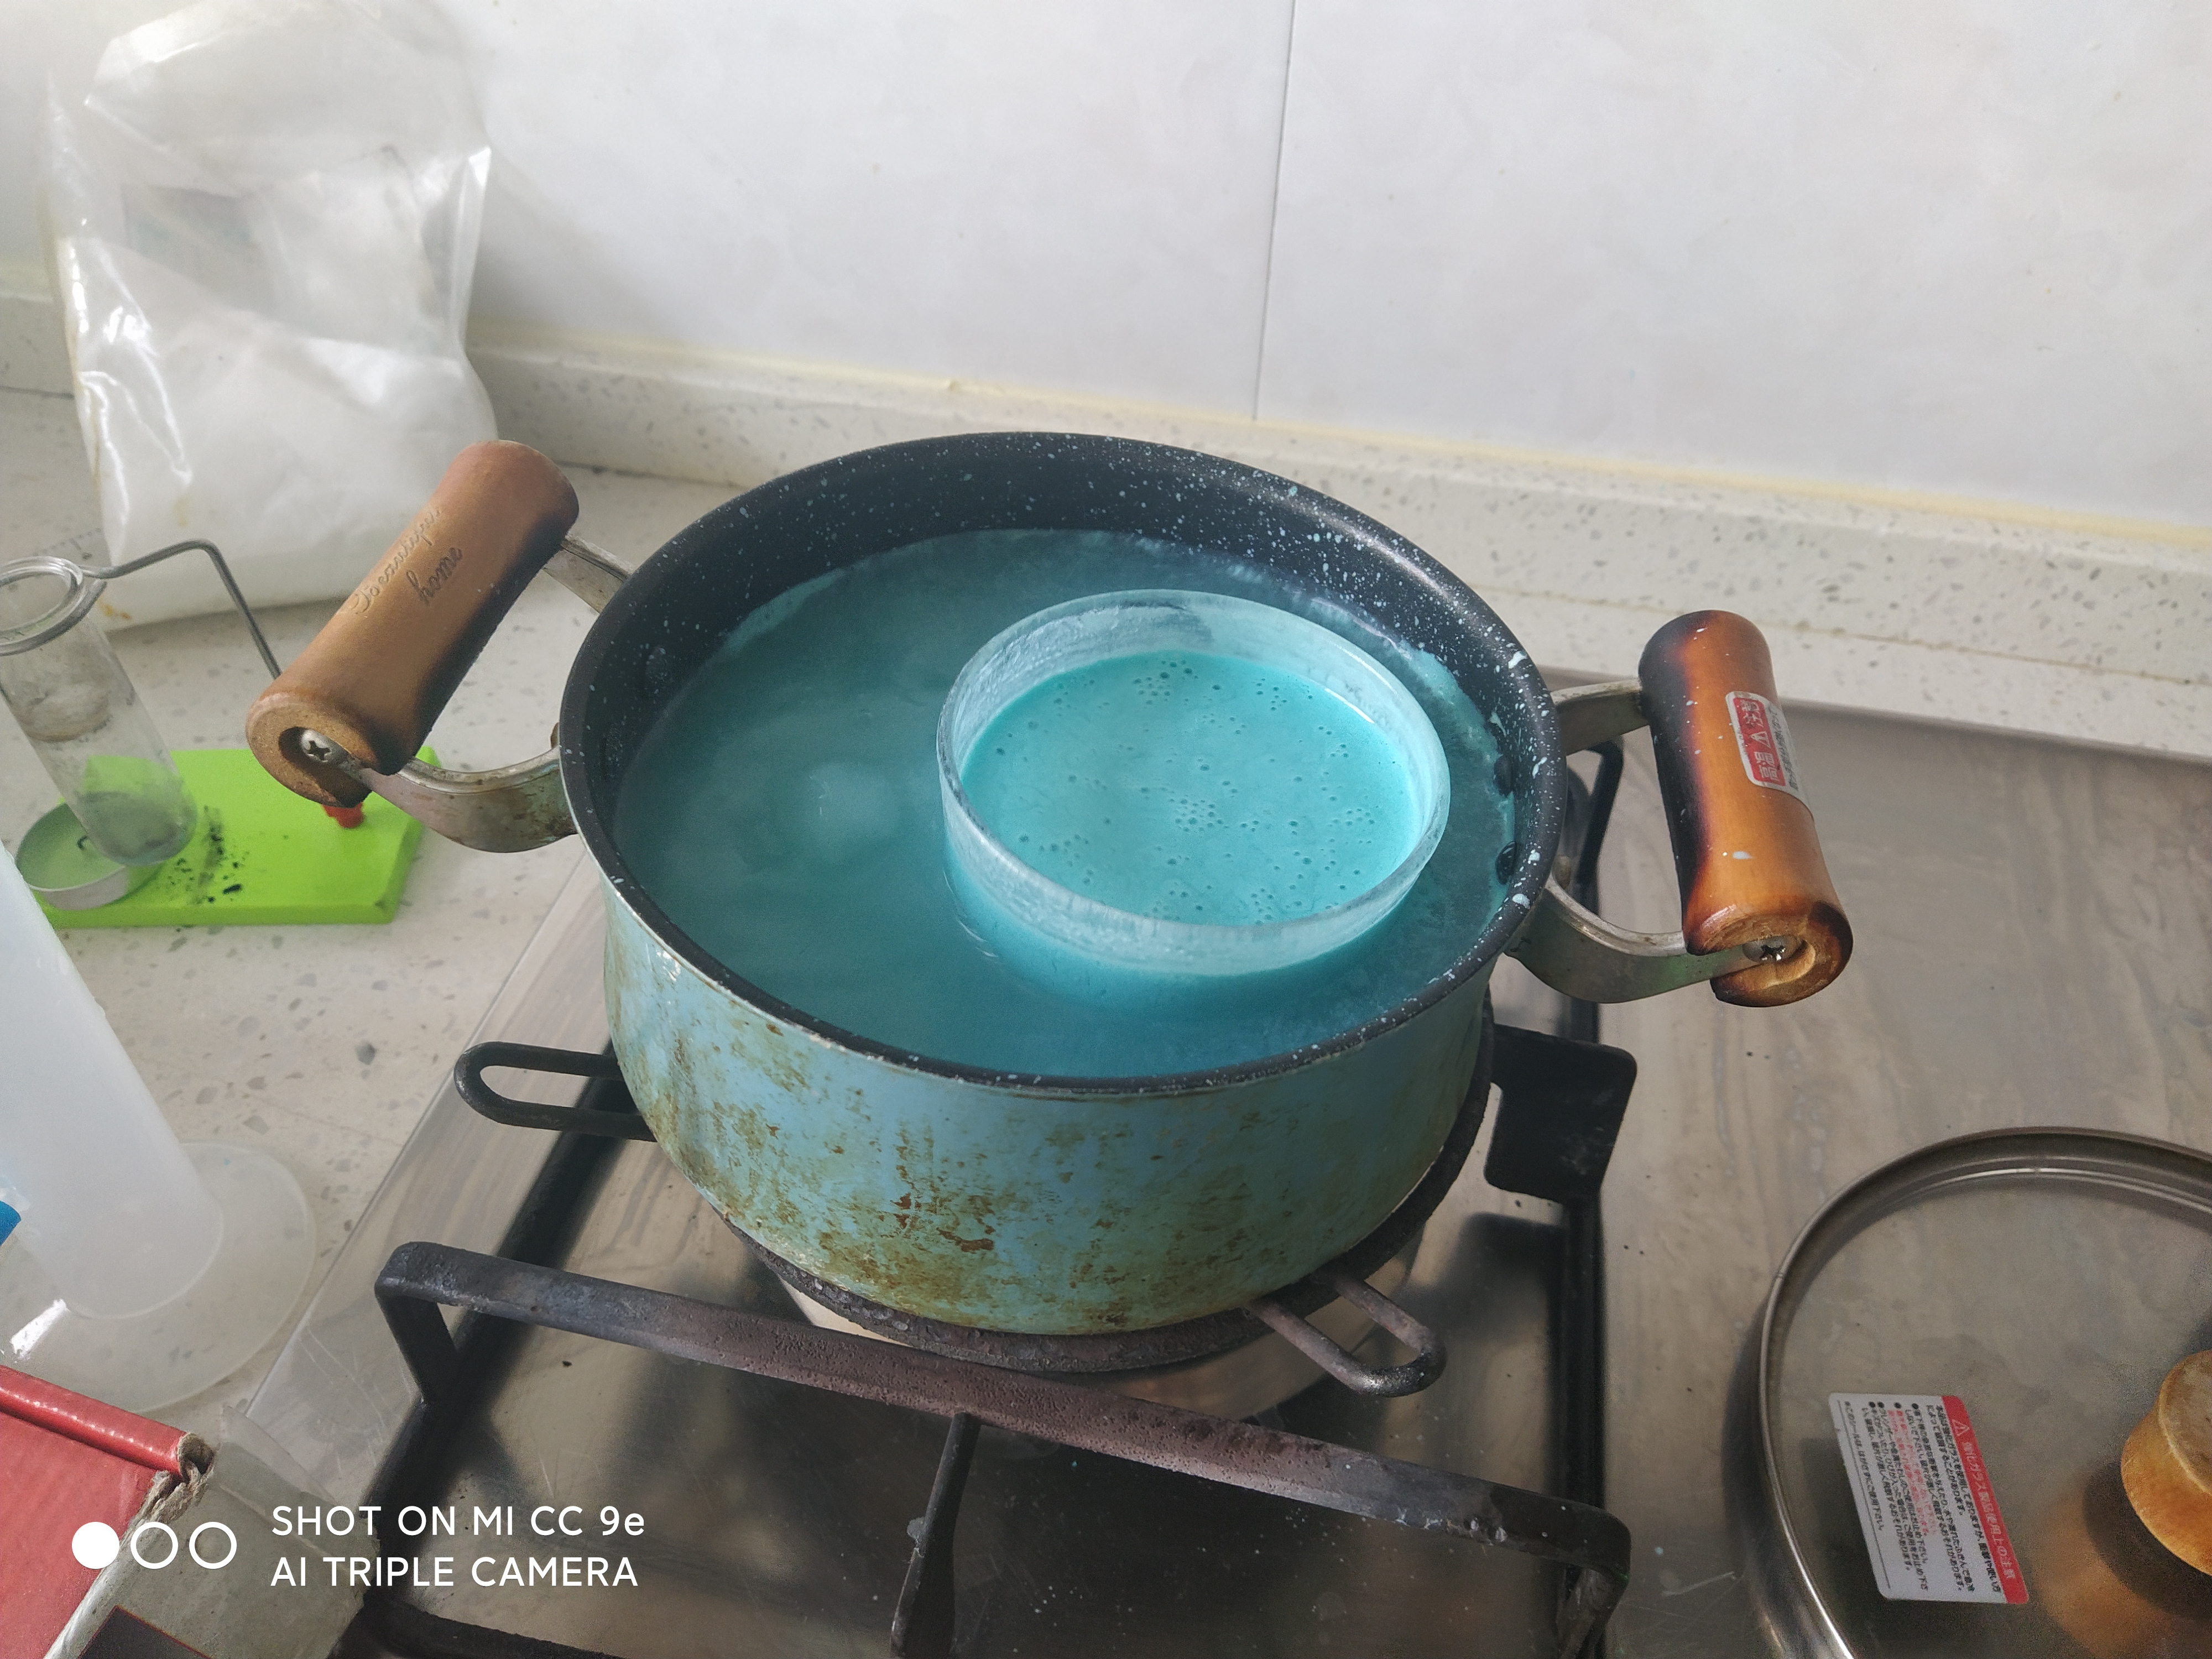
\includegraphics[scale=0.06]{photos/2During1.jpg}
\end{center}
\paragraph{
    反应越来越缓慢,到后来反应生成的二氧化碳不足以托起碱式碳酸铜,将其加热至上部
    清澈,便反应结束\\
}
\begin{center}
    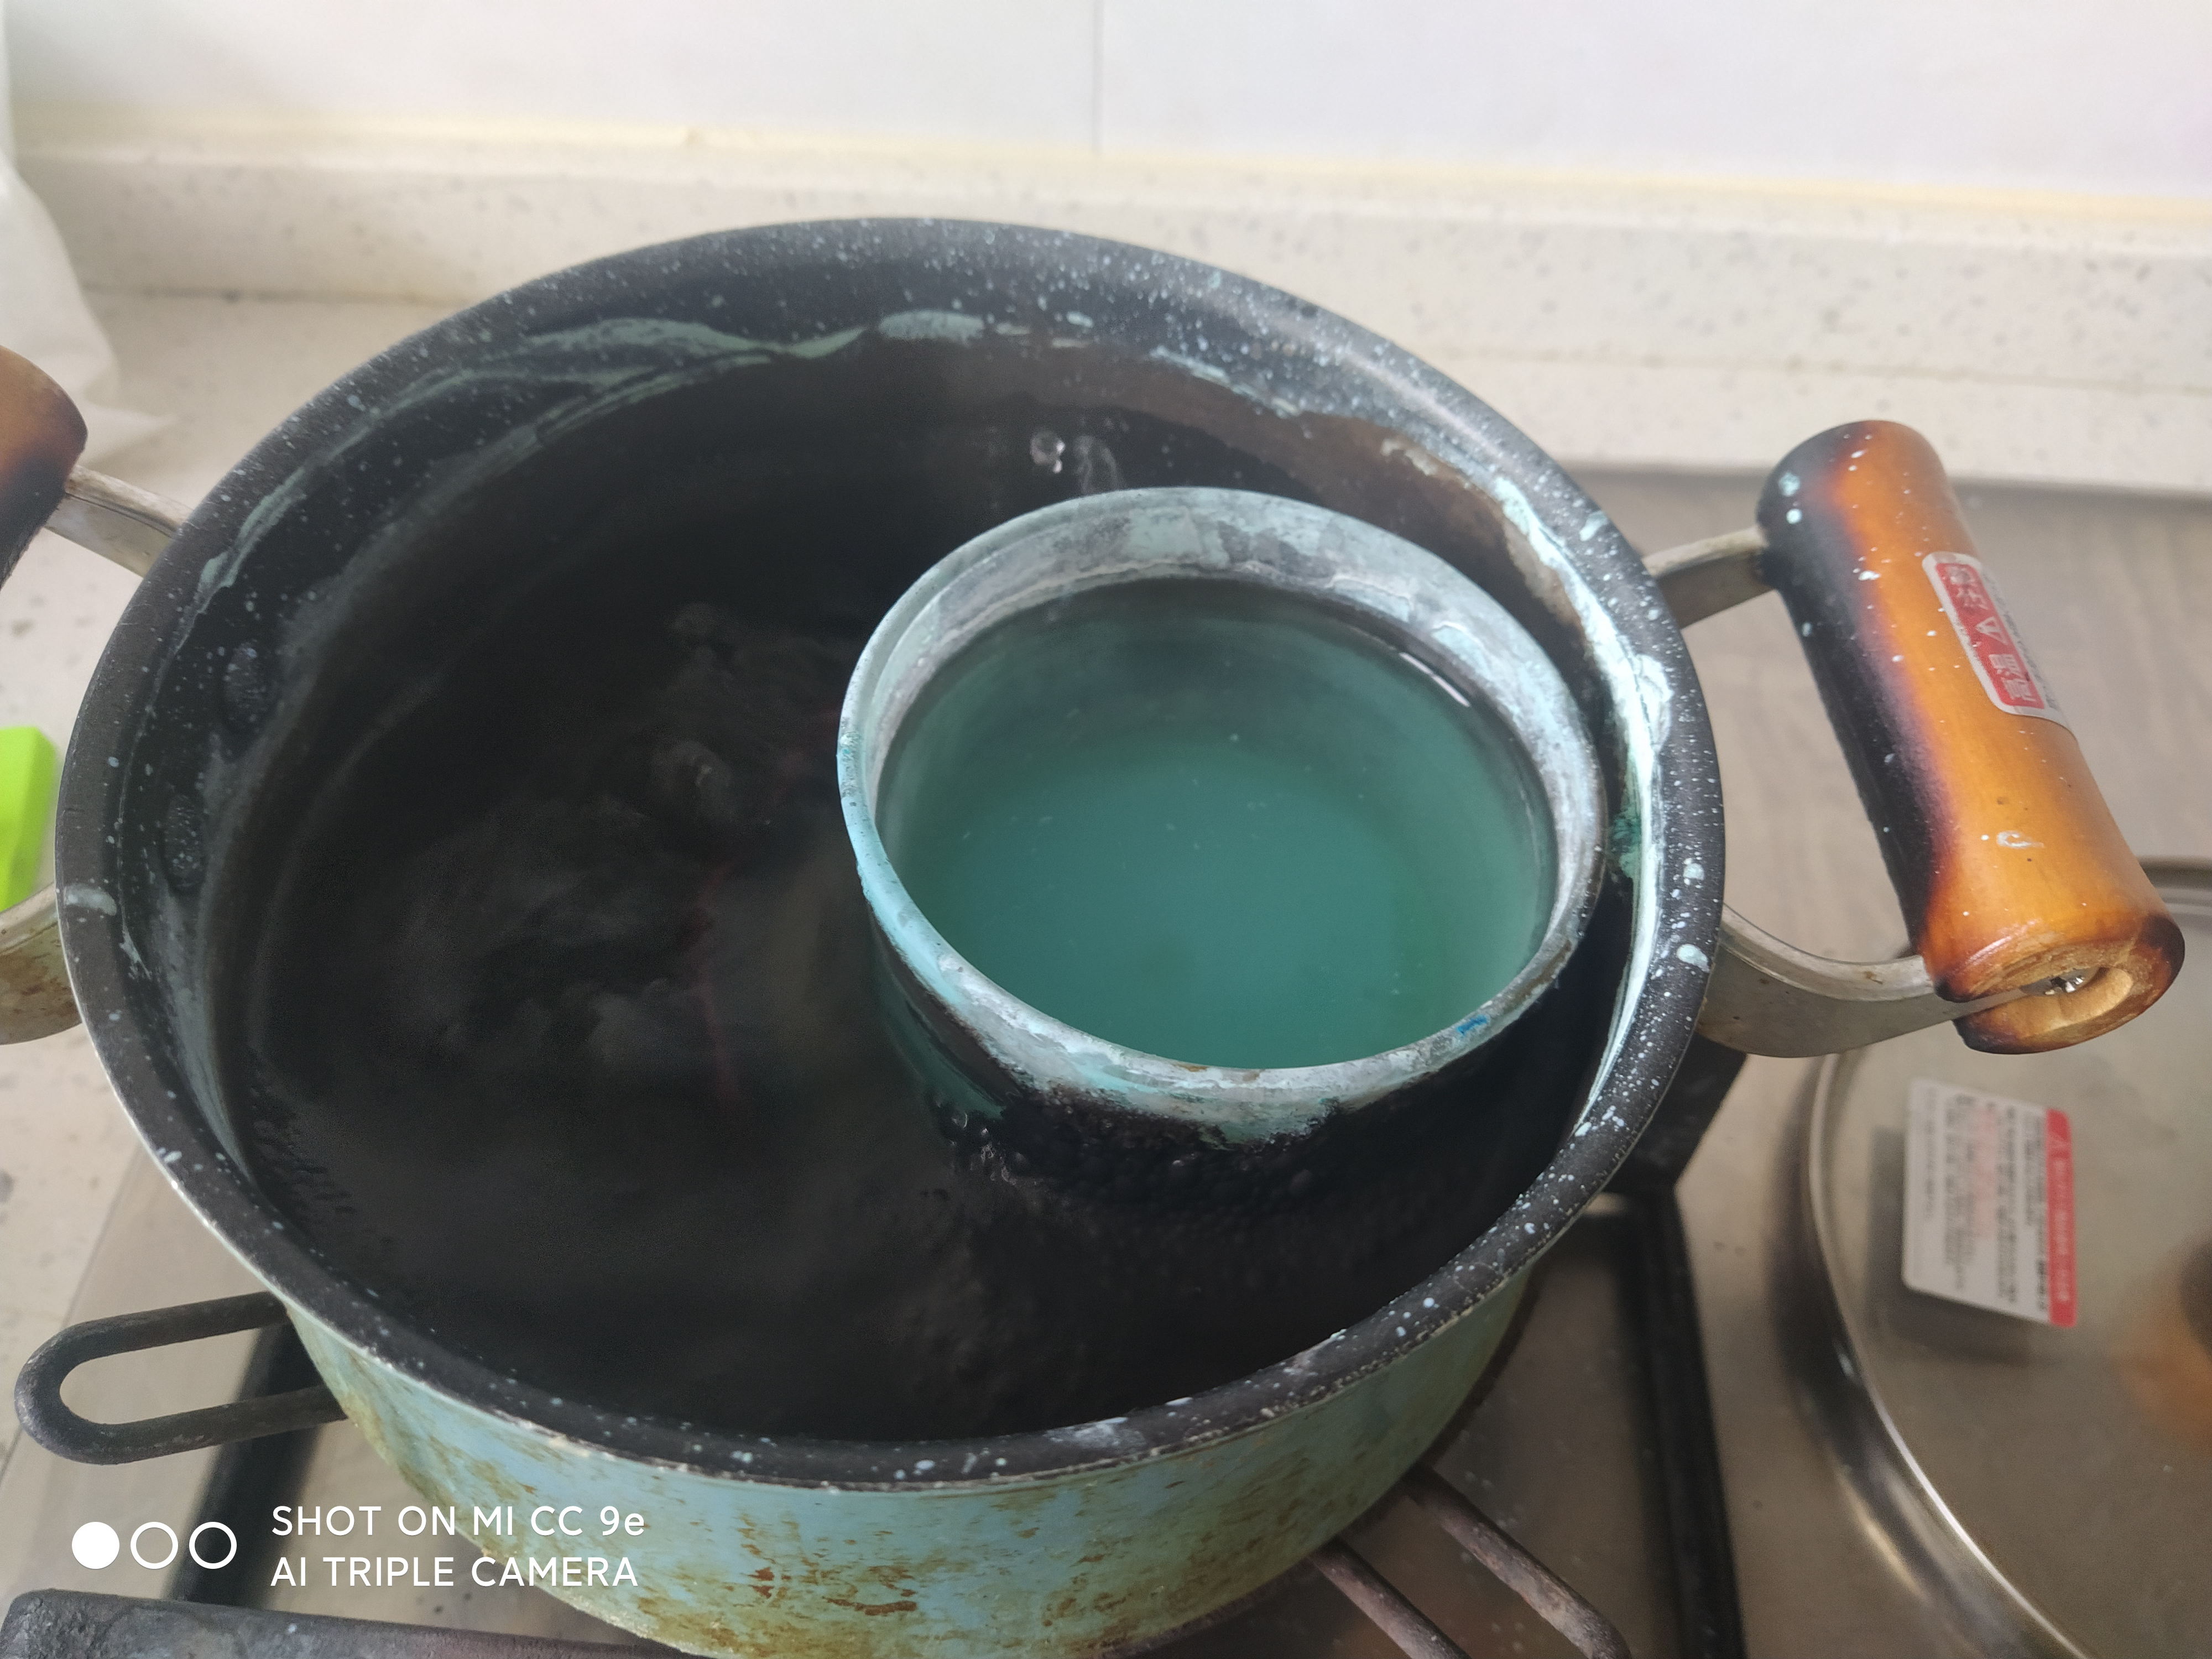
\includegraphics[scale=0.06]{photos/2DuringEnd.jpg}
\end{center}
\paragraph{
    该反应约进行45分钟\\
    将反应容器取出,用针筒抽走上部硫酸钠溶液(带有蓝色,说明硫酸铜仍过量,但是残余较少)。
}
\begin{center}
    \includegraphics[scale=0.3,angle=90]{photos/2End1.jpg}
\end{center}
\paragraph{
    加入酒精润洗,使得固体集中到一边,倒出过多的酒精,将固体放置太阳下等待自然风干\\
}
\begin{center}
    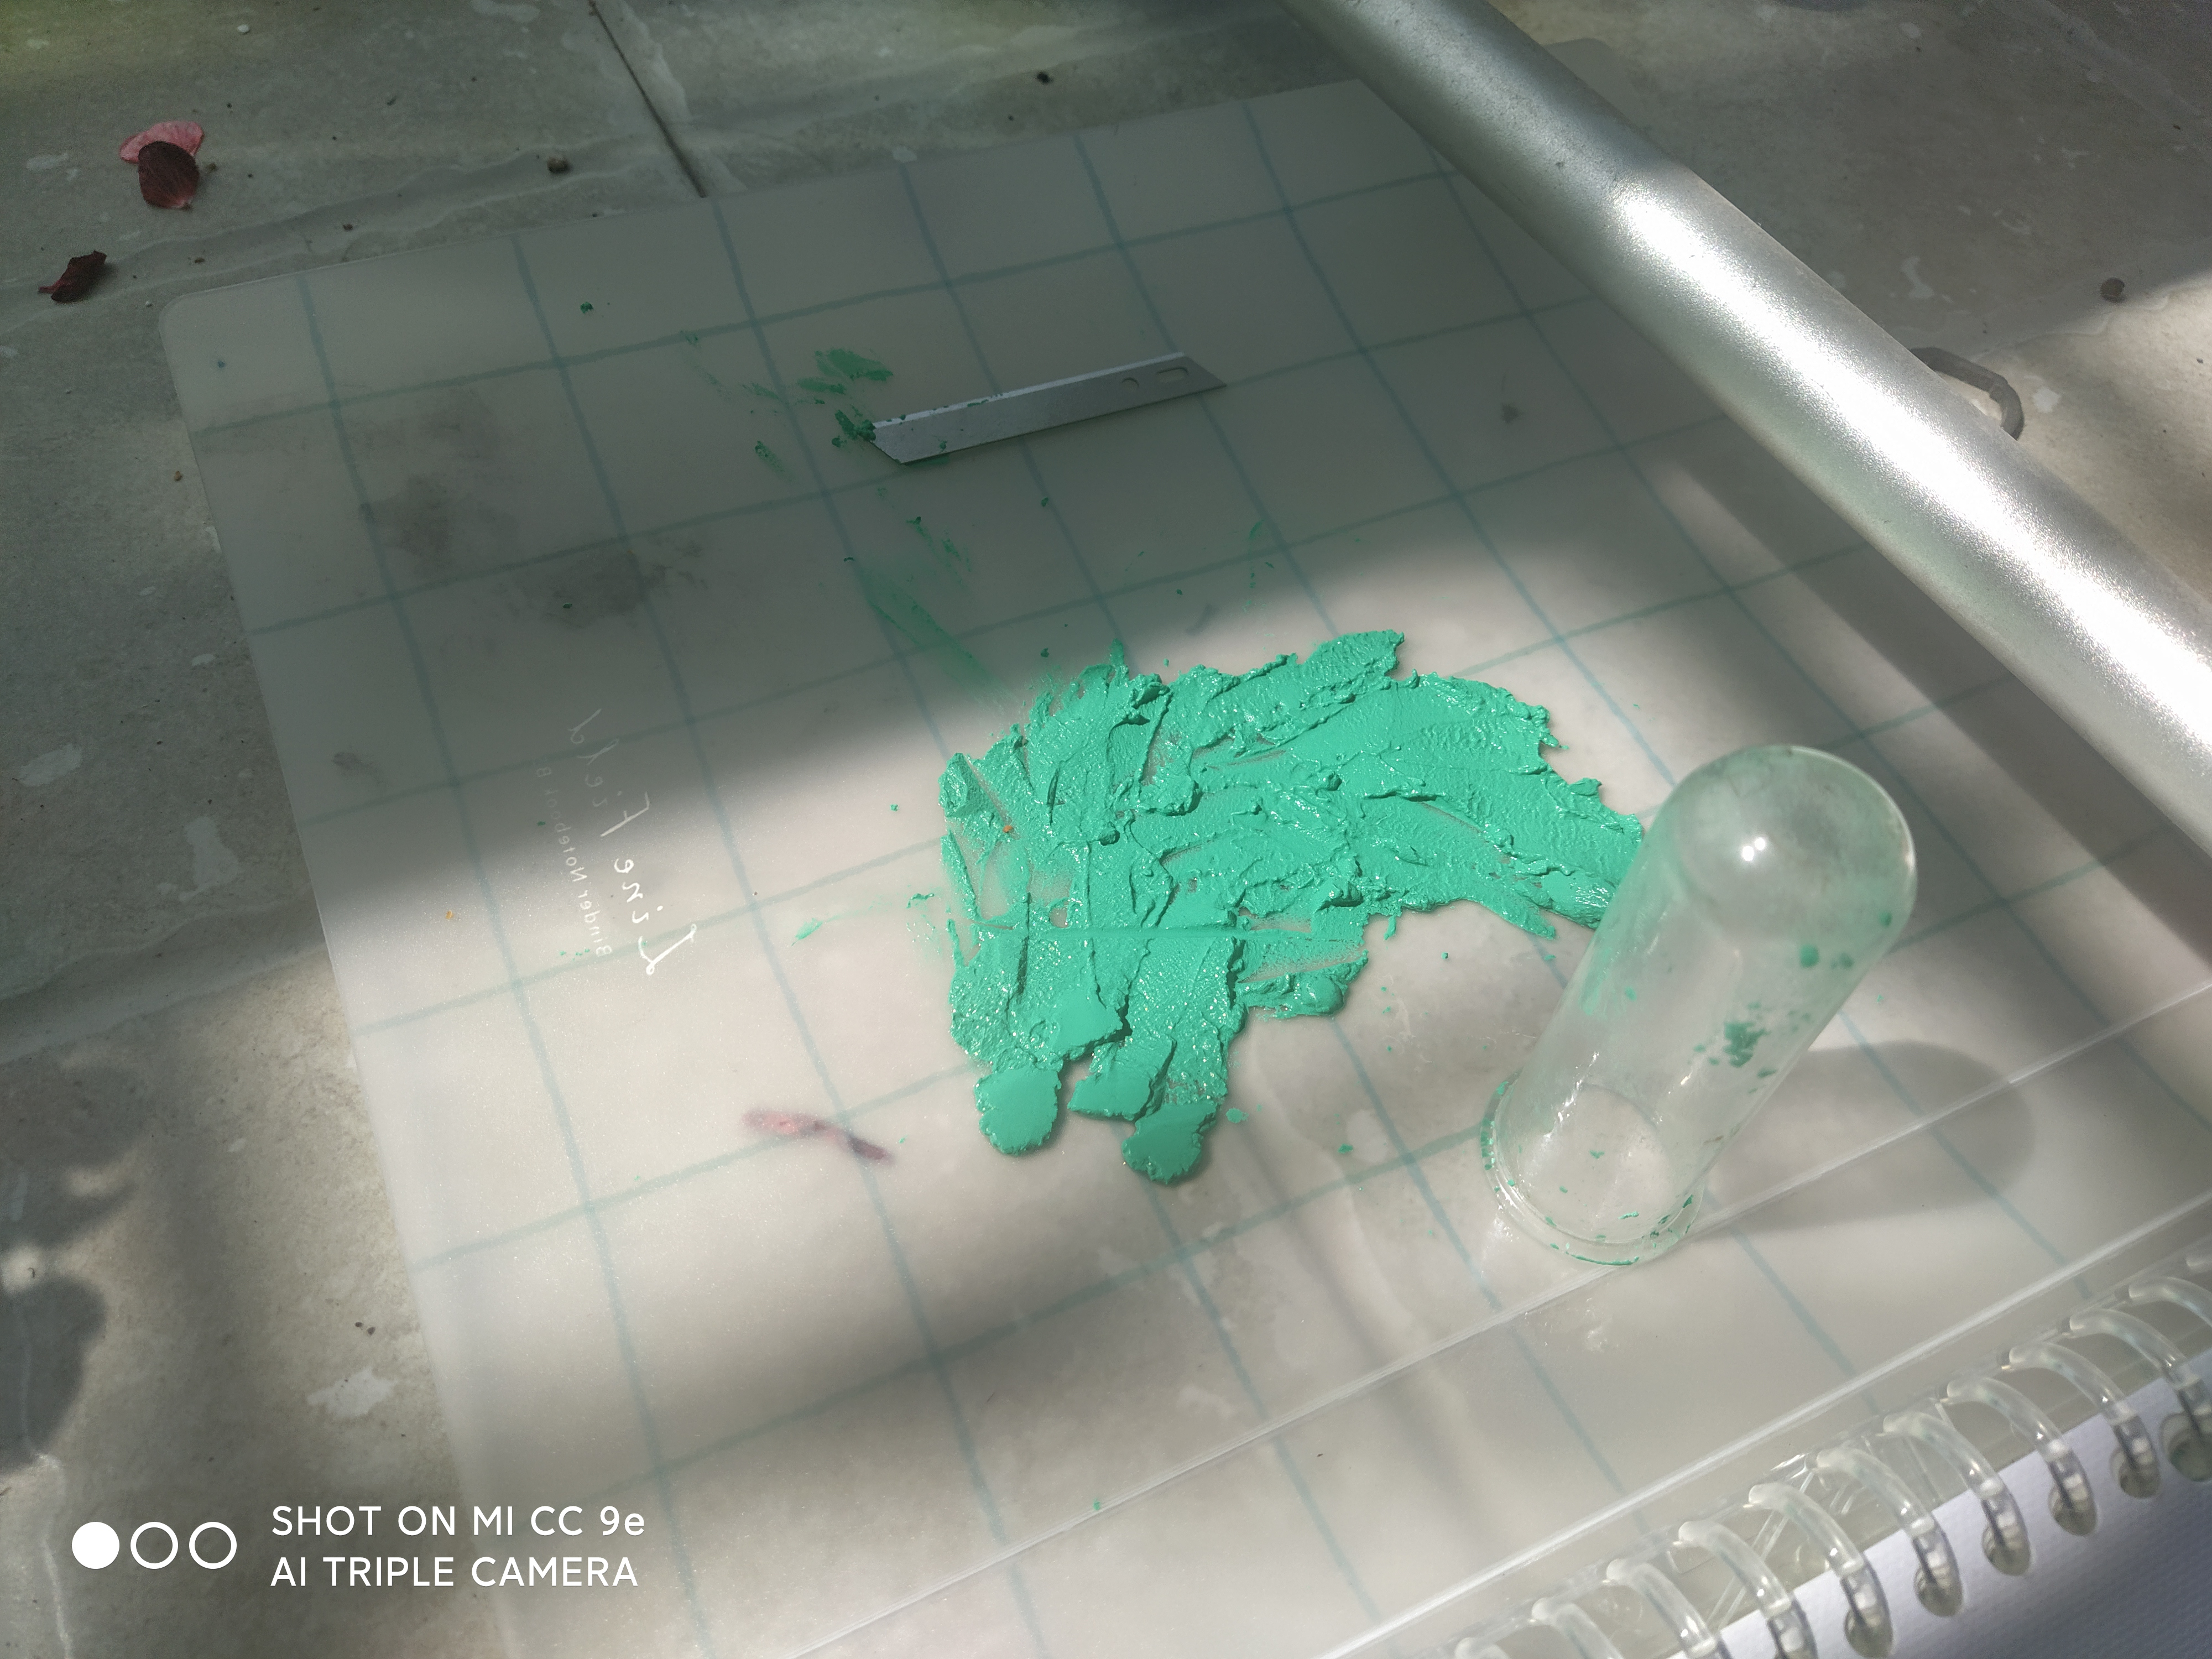
\includegraphics[scale=0.06]{photos/2EndDuring1.jpg}
\end{center}
\paragraph{
    理论生成5.525g\\
    称量产物量,实际生成产物5g\\
    产率90.5\%(由于产物中仍然带有水分,故产率实际小于该值)\\
}
\begin{center}
    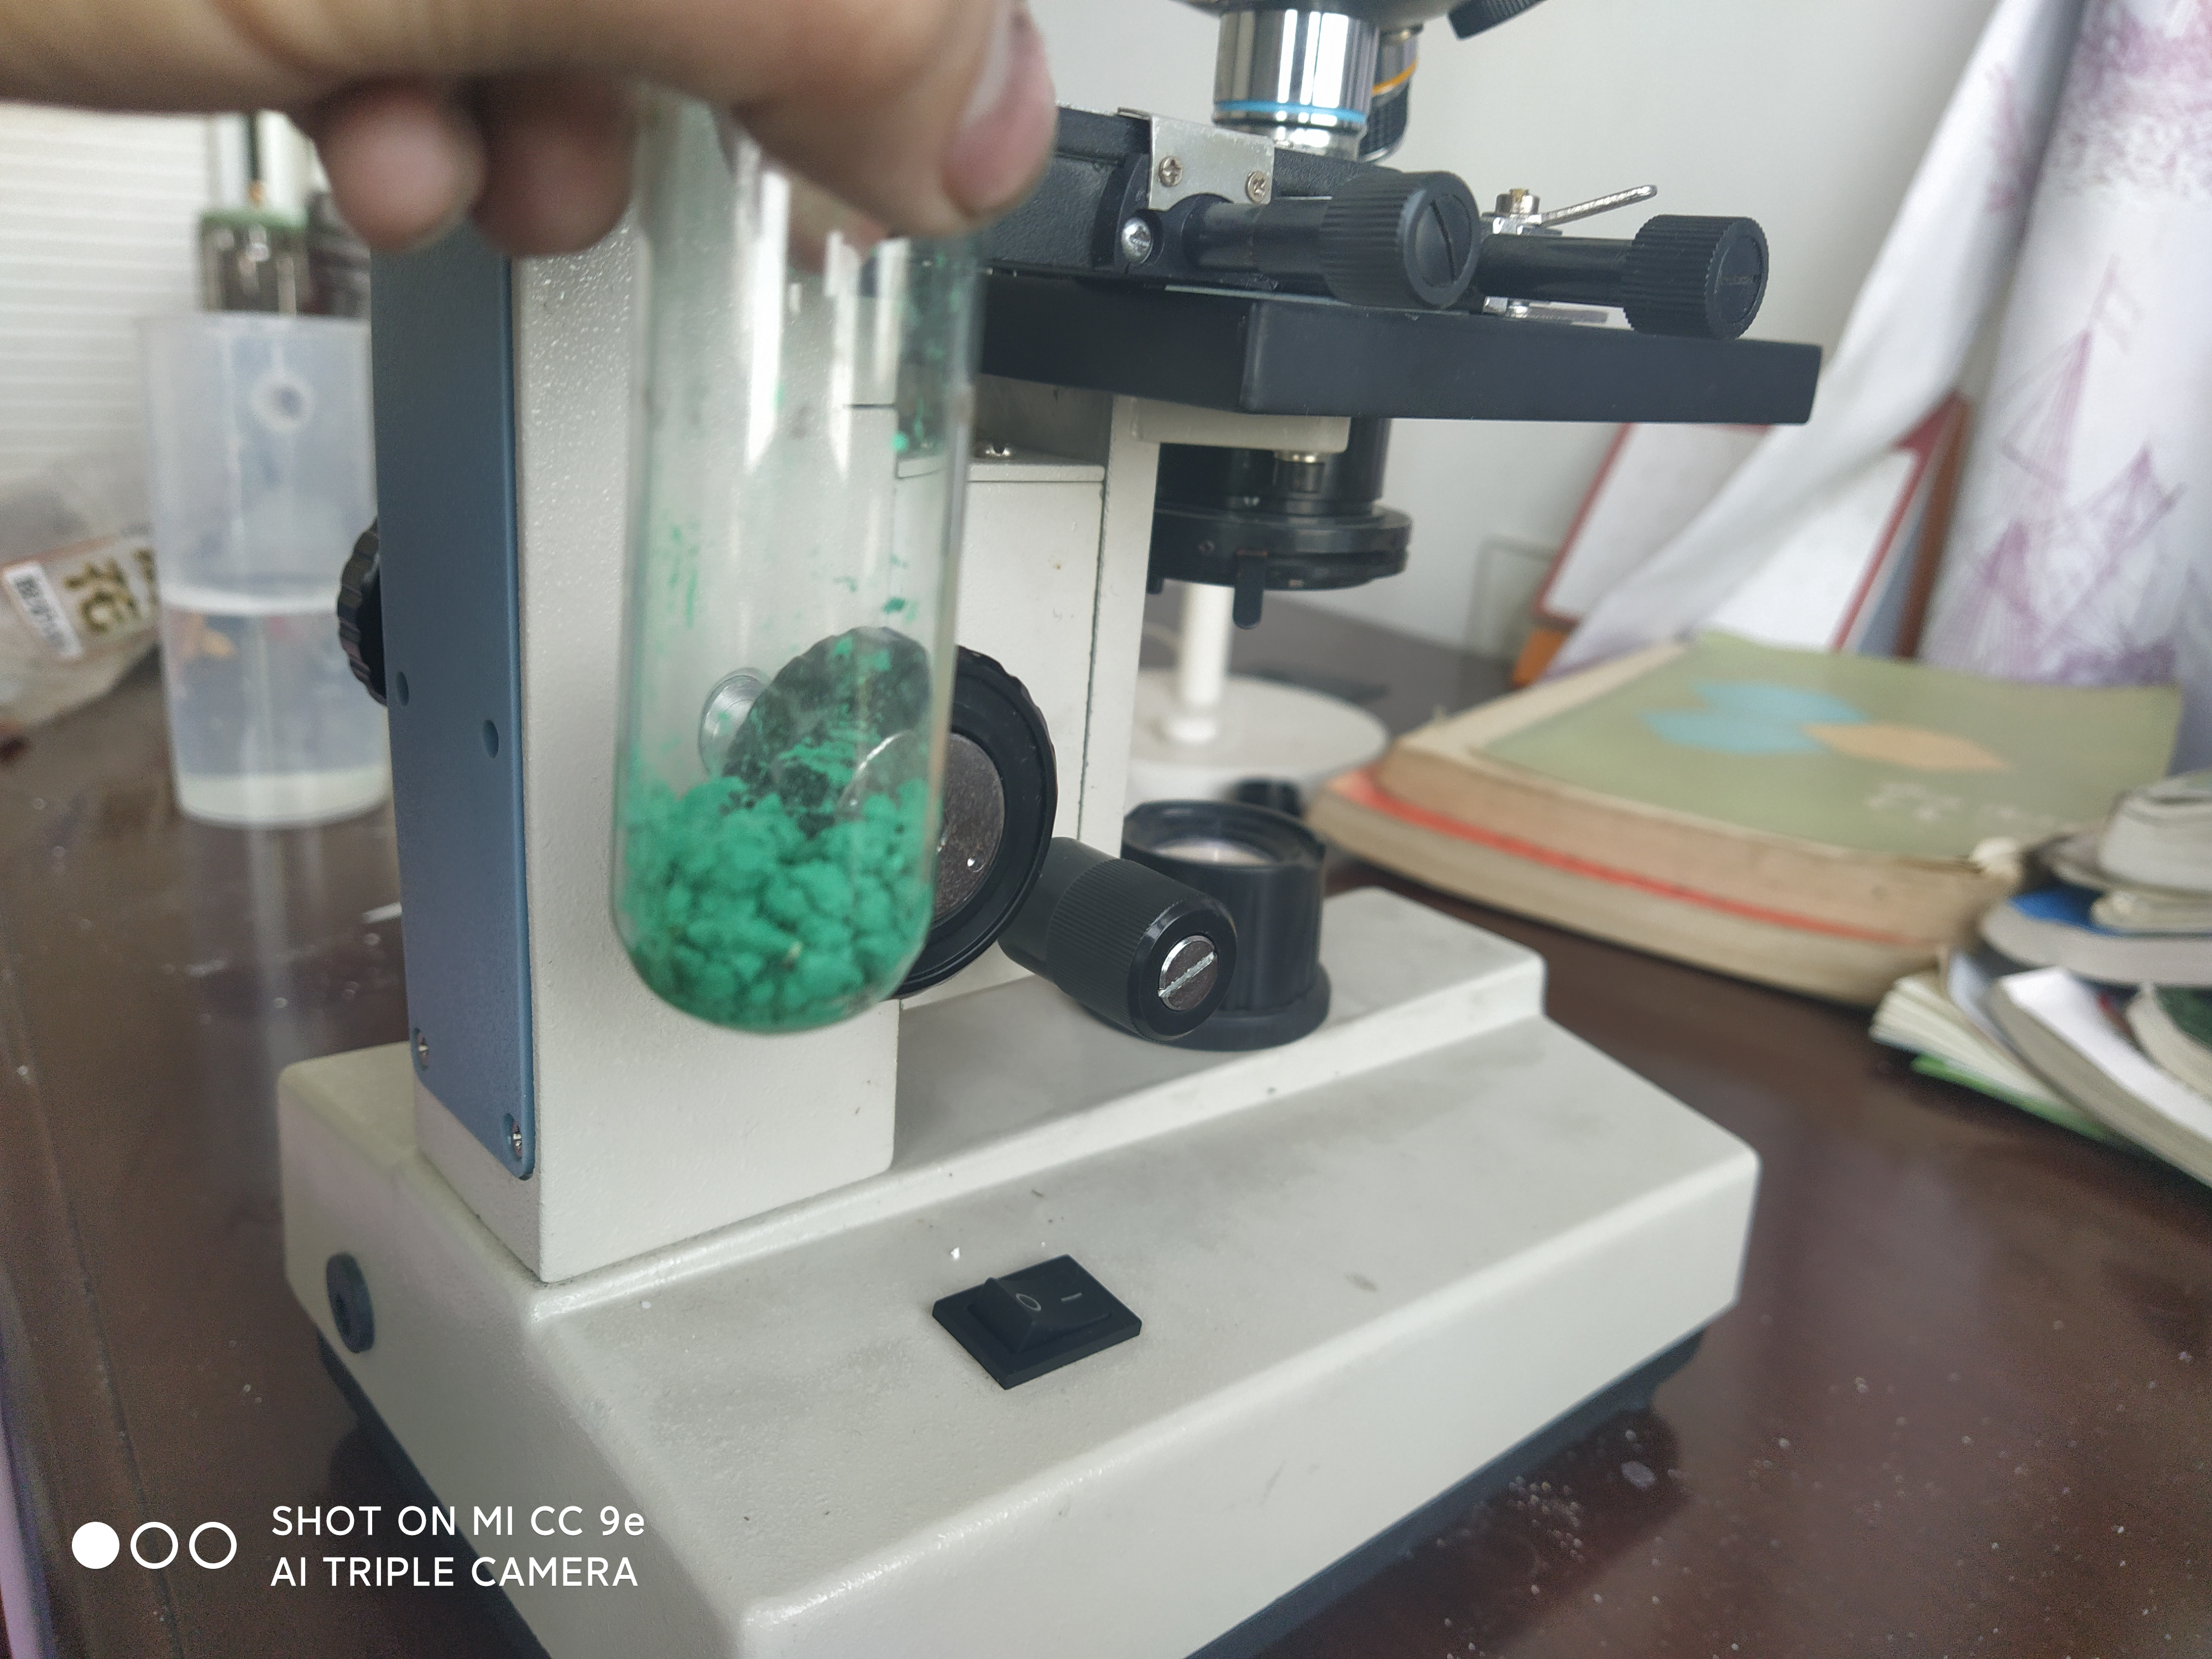
\includegraphics[scale=0.06]{photos/2EndEnd.jpg}
\end{center}
\subsection{实验结论}
\paragraph{
碱式碳酸铜是一种常用的工业原料,同时也是铜器表面的铜绿,孔雀石的主要成分,
工业中制取即使用硫酸铜和碳酸氢钠反应\\
由于碱式碳酸铜不溶解于水和醇,故可以用这个特性在水中反应,且可以使用乙醇
等较易挥发的物质脱去表面水。\\
碱式碳酸铜在镊子上灼烧时,碱式碳酸铜变黑,产生黑色物质,应为氧化铜,另产生二氧化碳和
水,这就可以解释第一次实验时上部黑色的物质\\
$$\ce{CuCO3 * Cu(OH)2 ->[$\Delta$] 2CuO + CO2 + H2O}$$
在这次实验当中,有效的锻炼了实验操作能力以及根据化学方程式计算的能力,且亲手研究
失败原因和反应过程中的各种各样现象,深刻理解了根据化学方程式计算的意义,这次实验是
一次非常有意思,也非常有意义的实验。\\
}
\section{总结与反思}
\subsection{实验不足}
\paragraph{
    实验完之后发现,底部不光有绿色的碱式碳酸铜固体,还是有蓝色的物质,故可能还是没
    反应完全,考虑一番之后,认为可能是硫酸钠在水中的溶解度不够大,反应到后来水中硫
    酸钠饱和,开始析出,故固体中可能存在有硫酸钠,反应不严谨。
}
\end{document}